\newpage
\section{Applicability of business intelligence to cryptomining data centers} \label{toc:ansatzmoeglichkeitenfuerbusinessintelligence}

In this chapter, the applicability of the principles of \ac{BI} processes to cryptomining data centers in order to achieve financial
optimization of the data centers will be evaluated. The goal of this part is to test the hypotheses presented in chapter
\ref{toc:hypothesenundabgrenzungderarbeit}. Thus, it is possible to finally make a statement about
the main hypothesis. In order to be able to formulate statements at the end, the methodology used is the
argumentative-deductive analysis. This methodology is qualitative in nature and belongs to the constructional science
methods.\footcite[Cf.][pp. 283]{wilde2007forschungsmethoden} Further statements are deductively derived from previous conclusions,
which in the end lead to the answer of the main hypothesis of this thesis.\footcite[Cf.][p. 7]{wilde2006methodenspektrum}
As a basis for the deduction, the elaborated foundations from
chapter \ref{toc:grundlagenbusinessintelligence} and chapter \ref{toc:grundlagenkryptomining} are used. In the first part
of this chapter, the \acp{KPI} from chapter \ref{toc:grundlagenkryptomining} are used in more detail and their origin is
considered. This fundamental data is analyzed according to various aspects, such as availability, real-time character,
quality, data change rate, and quantity, and thus their suitability for the \ac{BI} Processes is considered. The data
are subsequently subdivided according to internal and external sources. Finally, the reader will be able to understand which data is
available and how they are suitable for \ac{BI}. In chapter \ref{toc:pruefungderteilhypothesen} the actual testing of the
four sub-hypotheses is carried out. In the first step, the relevant \acp{KPI}
are identified, which are needed for the actual successful testing of the partial hypotheses. In the second step
the analysis procedures are examined to determine whether each of the relevant \acp{KPI} can be calculated from the basic data.
Finally, it is thus possible to verify the partial hypotheses and make a statement in chapter 
\ref{toc:zusammenfassendebetrachtung} at the level of the main hypothesis.

\subsection{Classification of available data} \label{toc:klassifizierungderdaten}

As described in the introduction to the main chapter, this part identifies and
categorized the available data sources. This categorization is used to determine the suitability of the data for \ac{BI}. The summary results
of this chapter can be found in table \ref{tbl:klassifizierunginternedaten} and table \ref{tbl:klassifizierungexternedaten}.

\begin{figure}[H]
    \caption{Classification of data sources}
    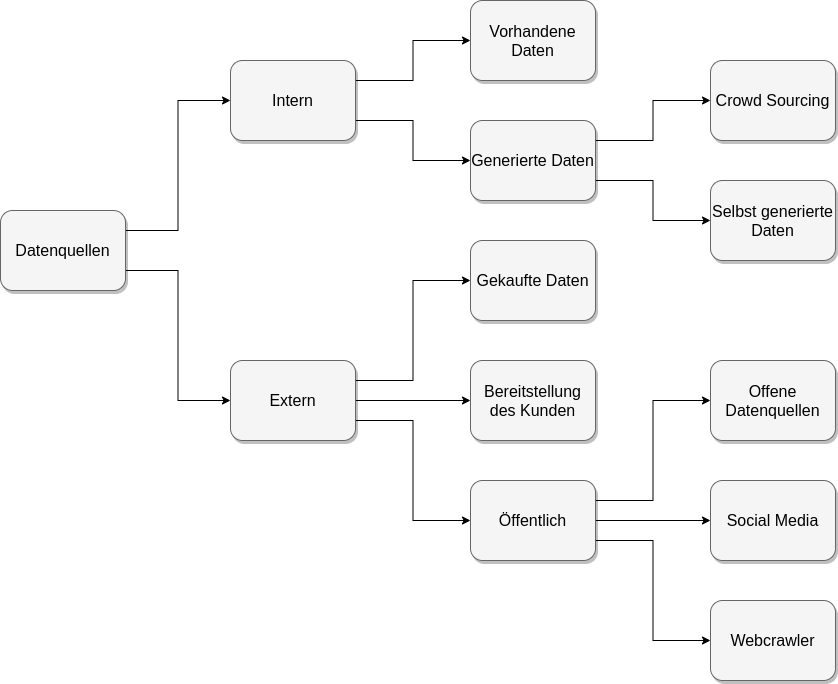
\includegraphics[width=0.7\textwidth]{datasources}
    \label{figure:datasources}
    \\
    \cite[Source: Based on][Fig. 1]{hartmann2016capturing}
\end{figure}

Based on Figure \ref{figure:datasources}, it is possible to divide the data into internal and external data sources at the first level.
This subdivision describes the origin of the data.\footcite[Cf.][Fig. 1]{hartmann2016capturing}
Internal data sources provide data that can only be accessed within an organization. These
data sources following include data from mining hardware, \ac{ERP} systems, and workforce planning. For the external
data sources, there is a three-part distinction between purchased data, data provided by a customer
and publicly available data. With this distinction, chapter \ref{toc:externedatenquellen} will primarily consider the
public data sources, since in the operation of cryptomining data centers the customer factor can be ignored for the time being.
These data sources include public block explorers, mining pools, exchanges, weather and climate data, as well as
data from social media platforms. The data is analyzed according to the following characteristics:
\begin{itemize}
    \item \textbf{Data structure: }Data can be divided into structured and unstructured data. Examples for
    structured data are financial data or sensor data.\footcite[Cf.][p. 27]{kimble2015big} Unstructured data
    can be images, text, or data from social media platforms.\footcite[Cf.][p. 27]{kimble2015big}This subdivision
    has an impact on the \ac{ETL} process, as data warehouses can only store structured data.\footcite[Cf.][p. 21]{niu2009cognition}
    In case of using unstructured data, it has to be adapted to become structured.
    \item \textbf{Availability: }This parameter measures the duration from the collection of a data point to its
    availability for users of the software. Especially for the analysis processes this parameter can have
    a big influence, as it determines whether a system is required that must process real-time data or, for example, only performs
    batch processing. The results from this category are used in the assessment of the eligible
    analysis processes in chapter \ref{toc:analyseverfahrenbi}.
    \item \textbf{Consistency: }This metric tells whether the data provided by the source systems,
    are free of inconsistencies. If data is not free of contradictions, this can lead to errors in the analysis processes and therefore
    must be observed closely.\footcite[Cf.][p. 561]{huh1990data} Since this has implications for the design of the analysis
    of the analysis processes, this fact must be taken into account.
\end{itemize}

\subsubsection{Internal data sources} \label{toc:internedatenquellen}

This part classifies the internal data sources and their data that can be considered for the design of a \ac{BI} process:

\begin{itemize}

    \item \textbf{Mining hardware / Monitoring software: }
    The technical parameters during operation are generated by the mining hardware. These parameters allow
    conclusions about the effectiveness of the hardware during the mining process. This includes data such as hashrate, temperature,
    hardware defects and power consumption.\footcite[Cf.][p. 12]{antminer2021manual} These metrics are available through \acp{API} or
    through the \ac{SSH} interface.\footcite[Cf.][]{awesomeminer2021api} As the configuration and monitoring of many individual
    devices represents too much effort and time consumption for personnel, software is used
    capable of monitoring and configuring a large number of mining devices. To achieve this,
    the \ac{API} or \ac{SSH} interface of the mining hardware is used. The use of the software can also reduce the
    mining hardware downtime and data center cooling power consumption can be measured. In addition
    this software is used by maintenance personnel to locate faulty equipment and repair it.
    The repair information is entered into the system by the personnel.
    \begin{itemize}
        \item Data structure: Since the data generated by the mining hardware and collected in the monitoring software is ultimately
        all sensor data, the data from this source is structured.\footcite[Cf.][p. 27]{kimble2015big}
        \item Availability: the availability of the data in the monitoring software is approximately five to ten minutes,
        as this data is retrieved via regular batch processes.
        \item Consistency: The consistency is given. All these data are stored in relational time series. 
    \end{itemize}

    \item \textbf{ERP System: }Financial \acp{KPI} are mostly stored in \ac{ERP} systems.\footcite[Cf.][Table 3]{spathis2003usefulness}
    These systems are used to maintain the financial \acp{KPI}
    of a data center. These data include acquisition costs, management costs,
    electricity costs and personnel costs. A detailed listing can be found in
    chapter \ref{toc:kennzahlenundeinflussfaktoren}. In the following considerations, these data are categorized as
    \ac{CapEx} and \ac{OpEx}, as this is sufficient for testing the hypotheses. Due to the interfaces
    of the ERP systems, this data can be queried uniformly.
    \begin{itemize}
        \item Data structure: since this data is primarily financial data and is queried through the interface
        of the ERP system, it is structured data.\footcite[Cf.][p. 27]{kimble2015big}
        \item Availability: once this data is entered into an \ac{ERP} system, it is also directly queryable.
        Therefore, an \ac{ERP} system provides real-time data.
        \item Consistency: Assuming that the incoming data is correct, the information from
        an \ac{ERP} system is free of contradictions and thus consistent.
    \end{itemize}
    \item \textbf{Staff planning: }Finally, workforce planning systems are available internally. These
    include the number of employees, their salaries and their working hours. In addition to the working hours, the
    shift schedules of the data centers are available in these systems, which can be used to draw conclusions about the staffing
    on site can be made. This data can be queried via standardized interfaces.
    \begin{itemize}
        \item Data structure: The data provided by the personnel system is structured and relational.
        \item Availability: The availability of such data can be queried directly and without delay as soon as it is entered in the system.
        entered into the system.
        \item Consistency: Assuming that all data entered is correct, all data in a
        personnel management system are free of contradictions.
    \end{itemize}
\end{itemize}

The following table lists the classifications of the individual data types that result from the above-mentioned data sources.

\begin{table}[H]
    \caption{Classification of internal data sources}
    \label{tbl:klassifizierunginternedaten}
    \begin{tabularx}{\textwidth}[ht]{X||c|c|c}
        Data Source & Data Structure & Availability & Consistency  \\
        \hline\hline
        Mining Hardware / Monitoring Software & Structured & 5-10 Minutes & Consistent \\
        \hline
        ERP System & Structured & \specialcell{Real-time within\\software} & Consistent \\
        \hline
        Personnel planning & Structured & \specialcell{Real-time within\\software} & Consistent \\
    \end{tabularx}
\end{table}

\subsubsection{External data sources} \label{toc:externedatenquellen}

Analogous to the classification of internal data in chapter \ref{toc:internedatenquellen}, the external data sources are classified in the following.
The following relevant external data sources are identifiable:

\begin{itemize}
    \item \textbf{Public blockexplorers: }Blockexplorers are websites that make the blockchain data accessible via interfaces.
    Examples of data that are directly on the blockchain are the Difficulty or even the amount of the
    transaction fees of the not yet confirmed
    transactions.\footcite[Cf.][]{bitcoin2021getdifficulty}\footcite[Cf.][]{bitcoin2021getrawmempool} In addition, there are
    metrics offered that can be calculated or estimated based on the data on the blockchain. These include
    data such as estimating the network hashrate of the Bitcoin
    network.\footcite[Cf.][]{blockchain2021total}\footcite[Cf.][]{blockchain2021api} Additionally, via such
    blockexplorer, any blockchain-related data can also be obtained in its full history. Another option,
    to obtain the blockchain data would be to operate your own Bitcoin node. Since the operation and maintenance of this
    requires a lot of expertise, querying the data through a public block explorer is preferable.
    \begin{itemize}
        \item Data structure: the nature of the data provided by a block explorer is structured.
        This is mainly due to the strict structured nature of the blockchain.
        \item Availability: Availability differs depending on the parameters queried. Data that is stored directly on
        the blockchain can be queried in real time. Examples include difficulty or information
        about transactions.
        
        All other data that is calculated on the basis of the blockchain data, but does not originate directly from it, is
        usually published only once a day. An example is the extrapolated total hashrate of the Bitcoin network.
        \item Consistency: Since the consistency of the data was one of the reasons for the introduction of blockchains,
        consequently, the data of a block explorer can also be considered to be free of contradictions and thus consistent. 
    \end{itemize}

    \item \textbf{Mining pools: }As already shown in chapter \ref{toc:miningundkonsensalgorithmen}, there is the
    possibility of participating in mining through mining pools. A mining pool offers the possibility of risk reduction
    during the mining process. In return, the mining pool charges user fees, which can be of different amounts.\footcite[Cf.][pp. 59]{bhaskar2015bitcoin}
    These fees can be directly collected from a mining pool
    and thus enter into the overall financial assessment. Since the owner of the mining hardware will be rewarded proportionately
    to the hashrate provided to the owner of the mining hardware, the incoming hashrate of a mining pool is traceable.
    This can be compared with the hashrate of the mining hardware to be able to make statements about the
    network connections. All this data is available in a standardized way via an \ac{API}.
    \begin{itemize}
        \item Data structure: Hashrate data is comparable to sensor data. For this reason, a
        mining pool outputs structured data.\footcite[Cf.][p. 27]{kimble2015big}
        \item Availability: Data is queryable with a delay of 15-30 minutes.
        \item Consistency: Data are consistent because they are collected on a time series basis. There may be
        differences to the hashrate of the mining hardware can be measured. However, these are not inconsistencies, but
        give conclusions about the connection quality between the data center and the mining pool.
    \end{itemize}
    \item \textbf{Exchanges: }Exchanges are used to exchange bitcoins earned through the mining process into
    fiat currencies. There are two main factors to consider here. One is the current exchange rate
    between \ac{BTC} and \ac{USD}. Secondly, the trading fees of an exchange must also be taken into account.
    All these values differ from exchange to exchange. Exchanges have extensive and
    performant \acp{API} to be able to trade with them very fast.
    \begin{itemize}
        \item Data structure: Exchanges offer structured data. Only this form of data allows very fast
        processing and analysis.\footcite[Cf.][p. 27]{kimble2015big}
        \item Availability: The exchange's interfaces provide data in real time.
        \item Consistency: Exchange data must be consistent or trading problems may occur.
    \end{itemize}

    \item \textbf{Weather and climate data: }Operators of cryptomining data centers are able to save energy costs by dynamically adjusting the
    cooling systems to the outside temperature. In order to take advantage of this savings potential
    interfaces are needed where current and historical weather data can be queried. One example of
    comprehensive interface is World Weather Online.\footcite[Cf.][]{wwo2021api} This interface requires a charge
    for use, as the provision of global weather data is complex.\footcite[Cf.][]{wwo2021pricing} Particularly in the case of a
    data center, the inclusion of climate data makes sense in order to estimate the power consumption and the dimensioning of the cooling systems.
    \begin{itemize}
        \item Data structure: Weather and climate data are provided in a structured way to enable a good analysis.
        \item Availability: According to World Weather Online, the data is provided in real time.
        gestellt.\footcite[Cf.][]{wwo2021api}
        \item Consistency: Consistency of data is important and within a platform it is. When querying
        multiple sources for weather data, inconsistencies may occur.
    \end{itemize}
    \item \textbf{Social Media: }In early 2021, it was observable that through social media platforms, the Bitcoin
    exchange rate was strongly influenced
    (Cf. Fig. \ref{figure:btctweets}).\footcite[Cf.][]{forbes2021musk}\footcite[Cf.][pp. 1]{ante2021elon} Therefore, in
    an assessment of exchange rates, the influence of social media can now no longer be ignored. In social media
    it is possible to determine a sentiment picture by analyzing hashtags, for example. Statements made by
    high-reach individuals or groups that influence exchange rates can be quickly analyzed.
    \begin{itemize}
        \item Data structure: Data from social media platforms is unstructured.\footcite[Cf.][p. 27]{kimble2015big}
        \item Availability: The availability of data via web scraping or \acp{API} is real-time.
        \item Consistency: Since social media platforms can basically be participated in by anyone, the data that can be
        can be analyzed is inconsistent.
    \end{itemize}
\end{itemize}

\begin{figure}[H]
    \caption{Bitcoin exchange rate compared with the number of tweets with hashtag \#bitcoin per day}
    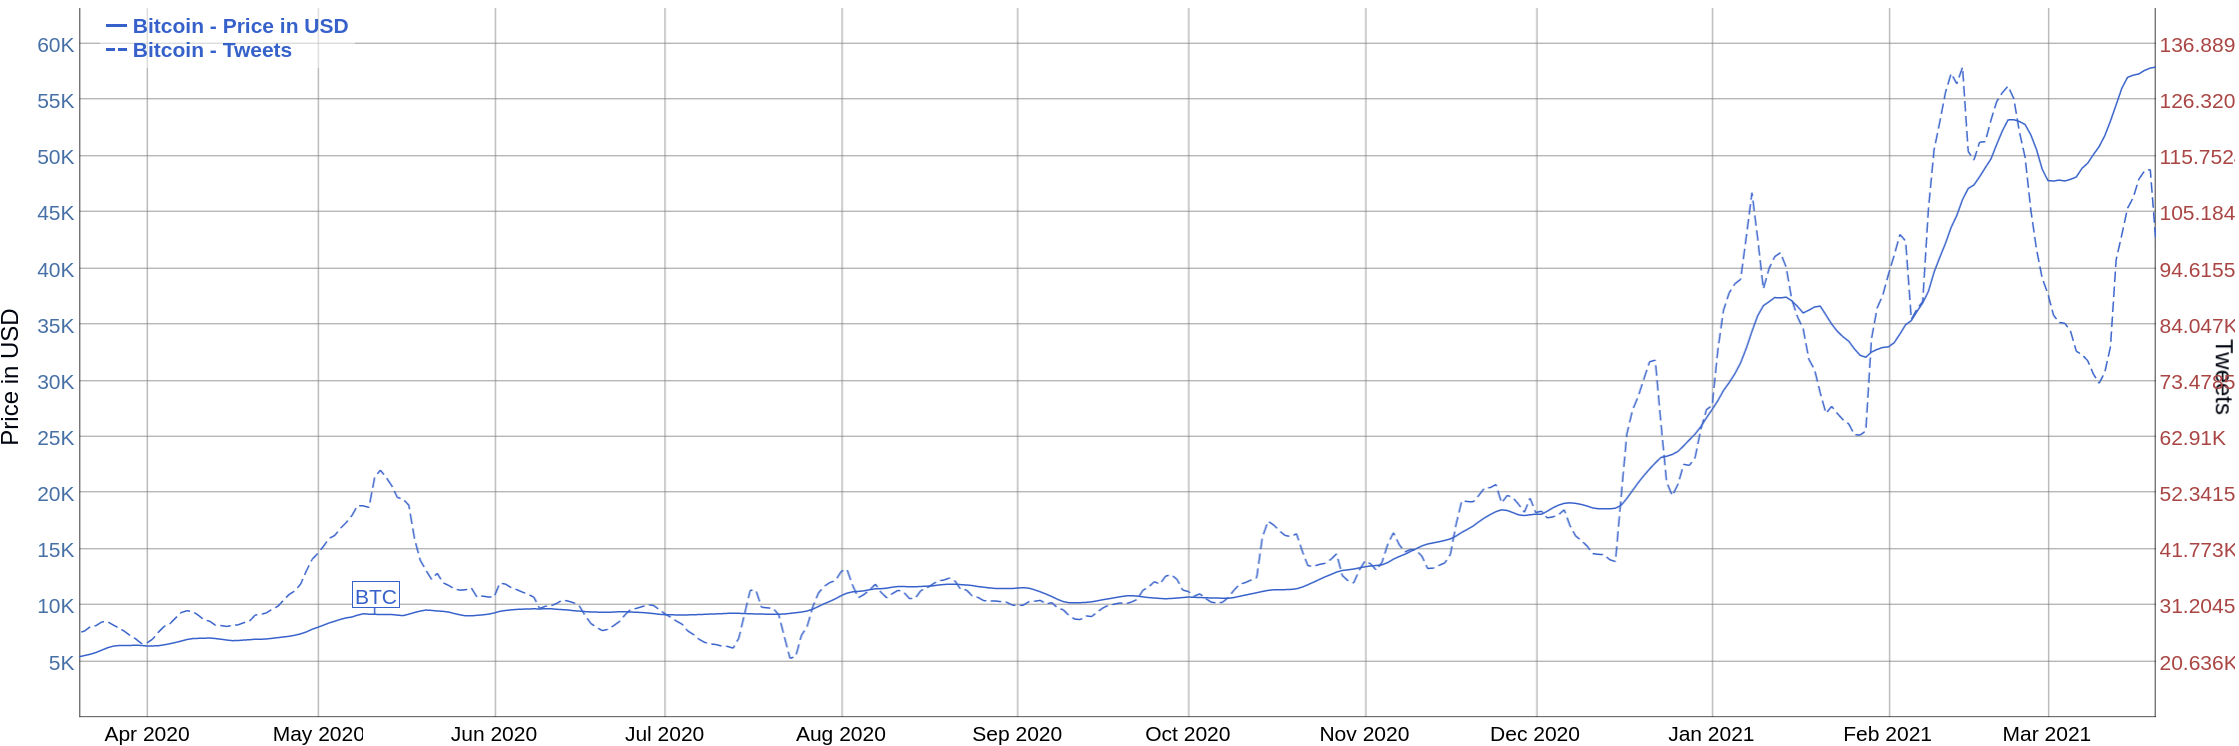
\includegraphics[width=\textwidth]{tweetsbitcoin}
    \label{figure:btctweets}
    \\
    \cite[Source: Cf.][]{bitinfocharts2021bitcointweets}
\end{figure}

In summary, the elaborated classifications are listed in table \ref{tbl:klassifizierungexternedaten}.

\begin{table}[H]
    \caption{Classification of external data sources}
    \label{tbl:klassifizierungexternedaten}
    \begin{tabularx}{\textwidth}[ht]{X||c|c|c}
        Data Source & Data Structure & Availability & Consistency  \\
        \hline\hline
        Public block explorer (blockchain data) & Structured & Real-time & Consistent \\
        \hline
        Public block explorer (metrics based on blockchain data) & Structured & 24 hours & Csonsistent \\
        \hline
        Mining Pools & Structured & 15-30 minutes & Consistent \\
        \hline
        Exchanges & Structured & Real-time & \specialcell{Consistent within\\any exchange} \\
        \hline
        Weather and climate data & Structured & Real-time & \specialcell{Consistent within\\any weather service} \\
        \hline
        Social media & Unstructured & Real-time & Inconsistent \\
    \end{tabularx}
\end{table}

\subsection{Testing of the sub-hypotheses} \label{toc:pruefungderteilhypothesen}

Based on the classification of the possible data sources and their available information, the testing of the partial hypotheses is carried out in this part.
For this purpose, it is defined for each individual sub-hypothesis which \acp{KPI} are relevant in order to evaluate and finally verify them.
For this purpose, the \acp{KPI} from the chapters \ref{toc:technologie} and
\ref{toc:miningrechenzentren} are used. In addition, the results will be compared across the available data sources from chap.
\ref{toc:klassifizierungderdaten} are included to identify data flows for a \ac{BI} implementation. These
will be used to answer the hypothesis. Figure \ref{figure:ht01dataflow} through \ref{figure:ht04dataflow} make it
it possible to check which data are needed, if they are usable for \ac{BI} and if they are available.
Chapter \ref{toc:analyseverfahrenbi} discusses which analysis procedures are needed for the data to ultimately
evaluate and test the sub-hypotheses. This will include a discussion of the different types of \ac{BI} - descriptive,
predictive, and prescriptive business intelligence - and their possible
limitations in the field of cryptomining.\footcite[Cf.][p. 96]{bihani2014comparative}

\subsubsection{Identification of the key performance indicators of the hypotheses} \label{toc:identifikationkpi}

As already written in the introduction to this chapter, this part identifies the data sources and the logical data flows.
For this purpose, all four sub-hypotheses are considered separately and a tailored dependency tree is defined for each of the
information and \acp{KPI} are defined. These are summarized in the respective figures that belong to the sub-hypotheses.
belong. In general, a distinction is made between financial, technical and personnel \acp{KPI}. Behind them are the
corresponding data sources from chapter \ref{toc:klassifizierungderdaten} are mentioned, which are of relevance. In the last level
the individual data types that are required are named. In the following, this analysis is performed for all four sub-hypotheses
carried out:

\begin{itemize}
    \item \textbf{\ac{HT0.1}: }This sub-hypothesis tests a possible influence of \ac{BI} on decision-making processes of the
    management regarding the construction or expansion of cryptomining data centers. Such decision support requires
    a large amount of data, as new construction or expansion is a complex strategic decision. For this reason, all
    three forms of \acp{KPI} - human, technical and financial - are needed.
    
    This strategic decision is based on factors regarding location, hardware selection, and the
    exchanges of bitcoin into fiat currencies to fund the data centers. The choice of location influences
    any forms of the \acp{KPI} already described, and thus is based on data such as staff salaries, \ac{CapEx}, \ac{OpEx}
    and energy consumption of mining hardware. The selection of hardware is in turn determined by factors such as hashrate, downtime
    (stability of the hardware), and energy consumption. The exchanges are significantly determined by the data that exchanges
    offer, to a large extent.
    
    According to table \ref{tbl:klassifizierunginternedaten} and \ref{tbl:klassifizierungexternedaten}, all these data are
    structured and consistent. Therefore, these data sources are readily suitable for use in \ac{BI} Processes.
    The \ac{ETL} process for each data source can be easily set up using the basic properties of the data mentioned above
    so that the data is made available by a data warehouse for the further sub-processes. The availability
    of the used data differs depending on the data type. In the case of exchanges, the data can be queried directly in real time.
    In contrast, technical \acp{KPI} have a delay of about five to ten minutes.  Systems like
    \ac{ERP} and personnel recording provide data in real time as soon as it is available to the system. Since strategic decisions,
    such as the construction or expansion of mining data centers are lengthy decisions, availability does not limit the hypothesis.

    Based on the data now available, the following chapter evaluates whether it is possible to analyze this data
    in such a way that in the end additional knowledge can be generated from it and thus these data can be used for decision support.

    \begin{figure}[H]
        \caption{Relevant KPIs, data sources and data types for sub-hypothesis 1}
        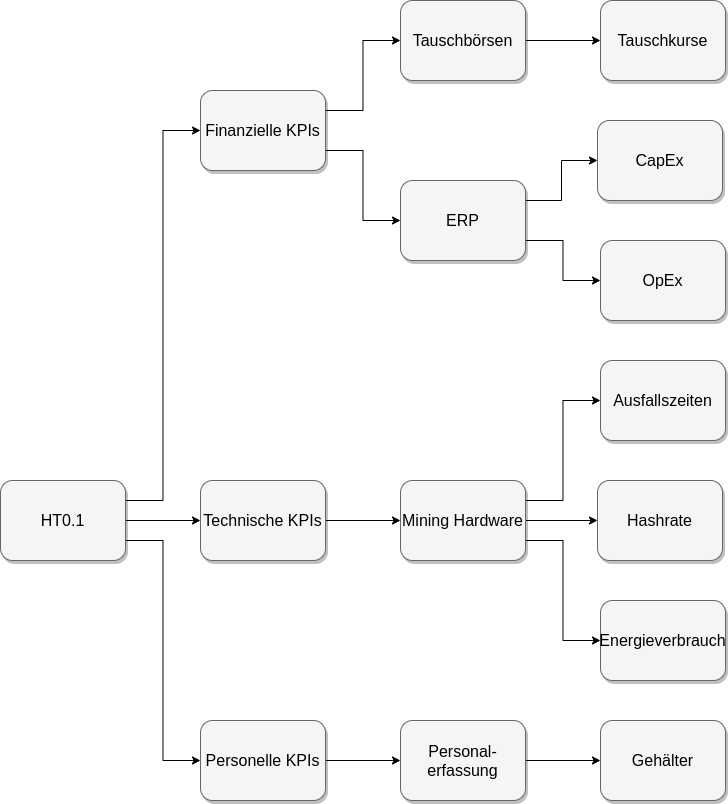
\includegraphics[width=0.55\textwidth]{ht01dataflow}
        \label{figure:ht01dataflow}
    \end{figure}

    \item \textbf{\ac{HT0.2}: }This sub-hypothesis deals with the influence of \ac{BI} on the effectiveness of the
    mining hardware. Since this hypothesis is exclusively technical in nature, only technical \acp{KPI}, such as
    power consumption, hashrate, downtime and hardware defects, are needed. This data comes exclusively from the
    monitoring system of the mining hardware. According to table \ref{tbl:klassifizierunginternedaten}, this data is both
    consistent and structured, making this data suitable for an \ac{BI} concept. The \ac{ETL} pipelines are
    easy to set up for this type of data. The delayed availability of the data (five to ten minutes) poses no
    problems for the hypothesis, since it does not necessarily rely on real-time data. Especially when measuring
    efficiencies in the mining process, one needs longer time windows of several days to obtain robust statements.
    Based on the data sources, factors can be calculated that have an influence on the effectiveness of the mining process.
    These include the hashrate of one's mining hardware, its energy efficiency ("Reference power effiency"
    $\frac{J}{TH}$) and the measurement of uptime and device defects, which for example can be optimized by better firmwares
    can be optimized.

    \begin{figure}[H]
        \caption{Relevant KPIs, data sources and data types for sub-hypothesis 2}
        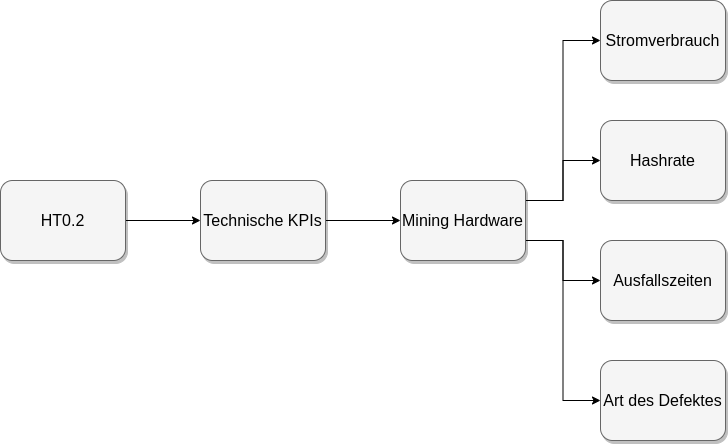
\includegraphics[width=0.55\textwidth]{ht02dataflow}
        \label{figure:ht02dataflow}
    \end{figure}

    \item \textbf{\ac{HT0.3}: }The third sub-hypothesis describes the improvement of the cash flow of a cryptomining
    data Center through the application of \ac{BI}. To test the hypothesis, technical and financial \acp{KPI}
    is needed. Among the technical \acp{KPI} are parameters, such as hashrate and information from public
    Blockexplorers, such as Difficulty and network hashrate projection. Through this information
    the theoretical mining yield can be predicted. The financial \acp{KPI} share in exchanges,
    \ac{ERP} systems, and mining pools. The exchanges provide data on their trading fees and exchange rates of
    \ac{BTC}. These are needed to exchange the received bitcoins into fiat currencies under the best possible conditions.
    to be able to do so. Another financial data source is \ac{ERP} systems, which provide a complete financial overview
    of all \ac{CapEx} and \ac{OpEx} items. Finally, mining pool information is still used (fees
    and revenue) to identify and use a pool with the highest possible payout. Using table
    \ref{tbl:klassifizierunginternedaten} and \ref{tbl:klassifizierungexternedaten}, all source systems, when properly
    use, all source systems provide structured and consistent data. As already noted in \ac{HT0.1} and \ac{HT0.2}
    noted, integration into a \ac{BI} Process is possible. Not all required data is provided in real time.
    provided. These include \acp{KPI}, such as mining pool fees and yields (15-30 minutes), network hashrate (24 hours)
    and mining hardware hashrate (five to ten minutes). Since cash flow is a financial measure that can only be calculated on large
    time spans (> 1 day), this delay does not pose a problem for the use of the data
    within an \ac{BI} process.

    \begin{figure}[H]
        \caption{Relevant KPIs, data sources and data types for sub-hypothesis 3}
        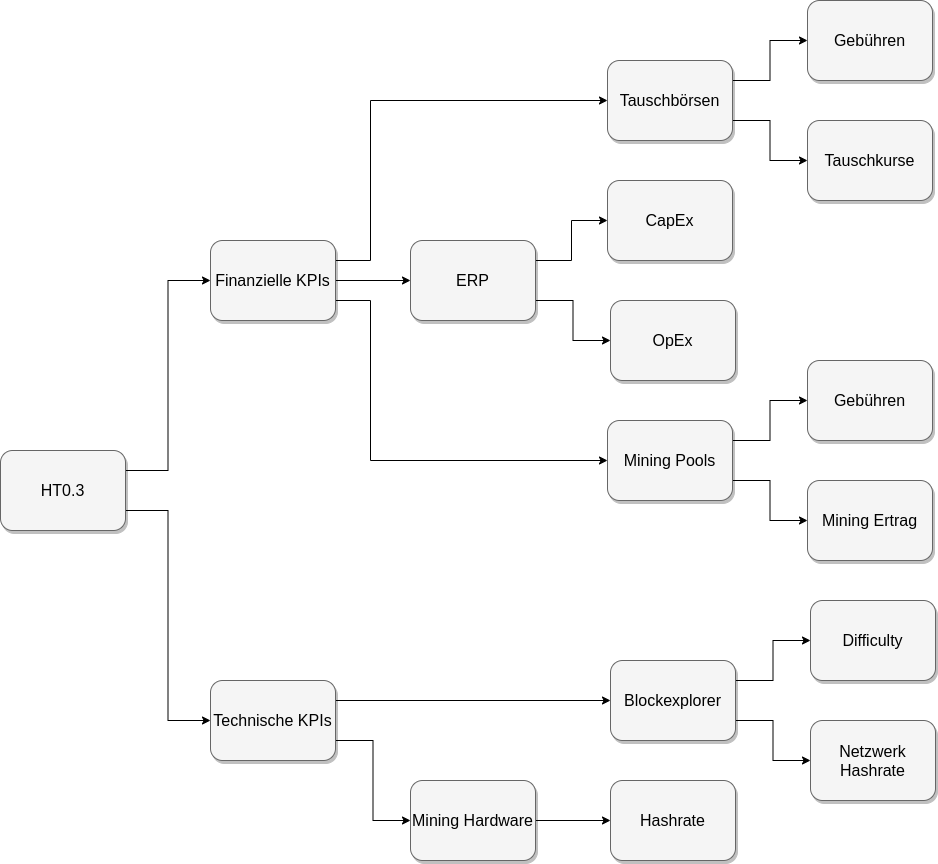
\includegraphics[width=0.7\textwidth]{ht03dataflow}
        \label{figure:ht03dataflow}
    \end{figure}

    \item \textbf{\ac{HT0.4}: }The last sub-hypothesis is in the area of human resource planning and states that this
    can be optimized by the application of a \ac{BI} process. To answer this hypothesis, both
    the technical \acp{KPI} as well as the human resource \acp{KPI} are relevant. Technical indicators include data,
    such as downtime and information about the nature of the hardware defect. Personnel \acp{KPI}, in turn, include data,
    such as shift schedules and staff training. By making these data sources available, it is possible to determine the
    average duration of a repair process and, on the basis of this, to make a realistic assessment of the on-site
    estimate the staffing levels on site. According to table \ref{tbl:klassifizierunginternedaten} all data are consistent and structured,
    which makes it possible to use this data in a \ac{BI}. The \ac{ETL} pipelines are readily feasible.
    However, the technical \acp{KPI} are only accessible with a delay of five to ten minutes. However, this represents
    for the feasibility of this hypothesis, because other data, such as new shift schedules, are updated only once a month and therefore the
    once a month and therefore the calculation of relevant results is not significantly affected by this delay.

    \begin{figure}[H]
        \caption{Relevant KPIs, data sources and data types for sub-hypothesis 4}
        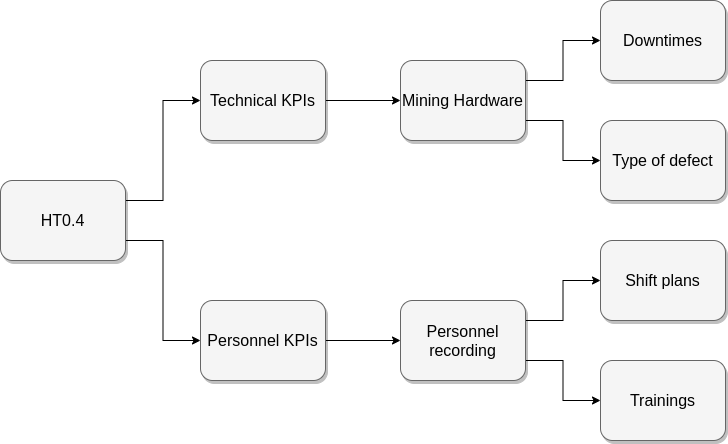
\includegraphics[width=0.55\textwidth]{ht04dataflow}
        \label{figure:ht04dataflow}
    \end{figure}
\end{itemize}

\subsubsection{Required analysis procedures within the business intelligence process} \label{toc:analyseverfahrenbi}

In order to be able to finally test the hypotheses, this chapter clarifies whether already established analysis processes are sufficient
to make the relevant data for a hypothesis usable in such a way that knowledge can be generated from it. In order to archieve this,
the existing analysis processes from the publication by Bihani and Patil are subjected to descriptive, predictive or prescriptive
paradigm of \ac{BI} and analyzed, whether the individual partial hypotheses can be
can be answered:\footcite[Cf.][pp. 97]{bihani2014comparative}\footcite[Cf.][Fig. 2]{bihani2014comparative}

\begin{itemize}
    \item \textbf{Descriptive analysis: }This item describes the analysis of past and already collected
    data. The following analytical procedures can be used for the descriptive approach\footcite[Cf.][pp. 97]{bihani2014comparative}
    \begin{itemize}
        \item \textbf{Factor analysis:}Through this form of analysis, underlying structures in the data are
        found out.\footcite[Cf.][pp. 97]{bihani2014comparative} To do this, large multidimensional data sets are
        reduced to smaller data sets that have explanatory power. These data sets thereby include
        fundamental factors, that can explain the measured large data sets.\footcite[Cf.][pp. 97]{bihani2014comparative}
        Such analyses are, among others, by means of \ac{OLAP} systems
        realizable. For answering the partial hypotheses, this form of analysis can be used. There exist
        in a data warehouse, which contains the data listed in chapter \ref{toc:klassifizierungderdaten}, large
        datasets, such as the hashrate of the mining hardware or exchange rates of \ac{BTC} to \ac{USD}. Also
        a comparison of these quantities is useful, such as of \ac{OpEx} and the overall hashrate of a data center.
        For these reasons, factor analysis and \ac{OLAP} systems can make sense for all sub-hypotheses.
        \item \textbf{Cluster Analysis: }This is an algorithm that can identify similarities in data sets.\footcite[Cf.][p. 98]{bihani2014comparative}
        This allows subsets of the data sets to be classified as contiguous.
        The umbrella term cluster analysis covers many algorithms that are known from the field of "data mining".
        These include the "K-Means algorithm" or "Nearest Neighbor".\footcite[Cf.][p. 98]{bihani2014comparative}
        The goal of using clustering algorithms to subdivide large datasets also provides an opportunity to structure
        the data to be further explored. Especially for technical \acp{KPI}, this form of analysis is therefore appropriate.
        Thus, cluster analysis is relevant to all sub-hypotheses and can be of help in the analysis. 
        \item \textbf{Discriminant function analysis: }The analysis can measure the difference between two measured groups of values
        and thereby determine whether a separation exists and how strong it is.\footcite[Cf.][p. 98]{bihani2014comparative}
        The application of this analysis is classically in understanding
        of demographic factors in the purchase of products.\footcite[Cf.][p. 98]{bihani2014comparative} Of interest is this
        form of analysis for interpreting identical \acp{KPI} from different data centers. It is precisely the analysis of
        differences of data between data centers enables the generation of new knowledge and is thus in the field of
        \ac{BI} of immediate relevance. The application of discriminant function analysis is therefore useful for all partial hypotheses
        useful as soon as more than one data center is considered.
        \item \textbf{Structural equation model: }In this process, dependencies between variables are formed and checked by means of linear
        equation systems to test whether this relationship actually exists.\footcite[Cf.][pp. 98]{bihani2014comparative} As
        result, the dependence or independence on the given model is determined.\footcite[Cf.][pp. 98]{bihani2014comparative}
        It is precisely to determine possible dependencies between the individual \acp{KPI} that this form of analysis can be used.
        A simple example is the dependency of the hashrate to the yield through the mining pool. Because of this
        the structural equation model also finds useful application in the present partial hypotheses.
    \end{itemize}
    In summary, it can be stated that there are a variety of different ways to analyze the present data
    and to generate knowledge for the stakeholders. With the help of the present forms of analysis
    a descriptive \ac{BI} process with the partial hypotheses is feasible.
    \item \textbf{Predictive Analysis: }In this paradigm, models for prediction are formed by means of various tools.
    Many of these tools come from the field of statistics and machine
    Learning.\footcite[Cf.][Fig. 1]{bihani2014comparative} The following forms of analysis are in addition to those already
    mentioned above:
    \begin{itemize}
        \item \textbf{Regression analysis: }This form of analysis tests the dependence of a variable on one or
        several variables.\footcite[Cf.][pp. 97]{bihani2014comparative} There are several forms of this, such as linear
        or logistic regression. This analysis can be used in forecasting profitability
        of market shares very well.\footcite[Cf.][p. 99]{bihani2014comparative} For this reason this form of analysis
        can be relevant for the sub-hypotheses to be tested. One application of
        regression analysis is the prediction of the value of bitcoins.\footcite[Cf.][p. 19]{ibrahim2020bitcoin} In principle
        a prediction using these mechanisms is quite possible. At the end of 2020, factors such as social media have been added,
        which make this form of analysis much more difficult.\footcite[Cf.][]{forbes2021musk} Accordingly, regression analysis can be a
        methodology to predict rates, but must be extended to include other analytical models to get a good
        overall picture. 
        \item \textbf{Stochastic analysis: }It is possible to simulate predictive models based on stochastic models.
        simulate. A well-known example of a stochastic analysis is the "Monte Carlo simulation". It can
        be used, for example, to estimate price developments and developments in the overall bitcoin hashrate for the future.\footcite[Cf.][p. 28]{cocco2016modeling}\footcite[Cf.][]{appendix:mcszenarien}\footcite[Cf.][]{appendix:mcpreis}\footcite[Cf.][]{appendix:mchashrate}
        Also with this form of the simulation, which was made on 06.11.2020, it can be determined that these are the developments
        of the Bitcoin price at the beginning of 2021 could not be predicted.\footcite[Cf.][]{appendix:btcusd} Therefore, this analysis model is not directly meaningful by itself,
        but must be supported by further modeling.
    \end{itemize}

    In the end, it can be stated that the Bitcoin price can only be predicted to a limited extent, as some influencing factors, such as
    social media, cannot be predicted and largely elude mathematical means of analysis.\footcite[Cf.][]{forbes2021musk}\footcite[Cf.][p. 325]{badertscher2017bitcoin}
    In general, however, this is not a problem exclusive to Bitcoin. In the case of traditional markets, the same
    problem is noticeable. However, due to the high volatility of the Bitcoin price, it is more noticeable in this case.
    In contrast, other \acp{KPI}, such as \ac{OpEx} costs or technical \acp{KPI}, are predictable, as they have
    little to no variation, and thus the results of descriptive analysis can still be used under this paradigm.

    Accordingly, it can be concluded that \ac{HT0.2} and \ac{HT0.4} are suitable for predictive models, as these exclusively use \acp{KPI}
    which can be simulated with sufficient quality. For \ac{HT0.1} and \ac{HT0.3}, predictive models can also be applied,
    where a limit can be established by predicting the bitcoin price. This can be improved by a suitable combination of the
    analysis models. If it is possible to suitably analyze the unstructured and inconsistent data from social media platforms,
    these should be integrated into the predictive modeling. To get the best possible impression of the \ac{BTC} price,
    it is important to work with real-time processing of this data.
    \item \textbf{Prescriptive Analysis: }This is the highest level that can be achieved using \ac{BI} processes. Thereby
    not only decision support is provided to the management, but decisions are directly recommended to the management by the system.
    The analysis of the hypothesis is similar to the point of predictive models, since this level of \ac{BI} is also based on these models.
    Accordingly, the result of this analysis is identical to the previous one and \ac{HT0.2} and \ac{HT0.4}. 
    As pointed out in the previous point, the other two hypotheses have limitations arising from
    the poor predictability of the bitcoin price. One possibility that the two partial hypotheses are suitable for the
    prescriptive analysis would be the calculation of different scenarios of the Bitcoin price and thus the calculation of
    different mining yields. Such predictive models already exist in-house through Monte Carlo simulation of the hashrate
    and the Bitcoin price.\footcite[Cf.][]{appendix:mcpreis}\footcite[Cf.][]{appendix:mchashrate}
    Since the answer to the feasibility of such a system is difficult to give in the course of this argument, it is
    this is considered in more detail in the case study in chapter \ref{toc:planungeinesbiprozessesfuereinminingrechenzentrum}.
\end{itemize}

Outside of this list, there are additional forms of analysis, such as compound analysis.\footcite[Cf.][p. 97]{bihani2014comparative}
This is used, for example, in analysis of customer buying behavior. Due to no relevance found for the use case of cryptomining
Data centers, this form is not considered further.

Table \ref{tbl:hypothesenanalyse} summarizes the visualization of the results of the previous analysis.

\begin{table}[H]
    \caption{Possible forms of analysis of the hypotheses}
    \label{tbl:hypothesenanalyse}
    \begin{tabularx}{\textwidth}[ht]{X||c|c|c|c}
        & \ac{HT0.1} & \ac{HT0.2} & \ac{HT0.3} & \ac{HT0.4}  \\
        \hline\hline
        Descriptive analysis & \checkmark & \checkmark & \checkmark & \checkmark \\
        \hline
        Predictive analysis & (\checkmark) & \checkmark & (\checkmark) & \checkmark \\
        \hline
        Prescriptive analysis & (\checkmark) & \checkmark & (\checkmark) & \checkmark \\
    \end{tabularx}
    \begin{tablenotes}
        \item \hspace{1mm}\checkmark\hspace{10mm} Feasible
        \item (\checkmark)\hspace{8.5mm} Feasible under the described limitations
    \end{tablenotes}
\end{table}

With the conclusion of this chapter, it is clarified whether the introduction of an \ac{BI} process is possible for the respective sub-hypotheses.
Finally, in the next chapter, the results of the four sub-hypotheses are used in order to obtain a first statement about the main hypothesis
and thus to answer for the first time the research gap that this thesis aims to fill.

\subsection{Summarized view} \label{toc:zusammenfassendebetrachtung}

After testing the individual sub-hypotheses in chapter \ref{toc:analyseverfahrenbi},
in this part this knowledge is used to obtain a statement about the main hypothesis.

There exist four stages that can be reached when analyzing data. These levels can be found in Figure
\ref{figure:levelofanalysis}. In the following, the relevance of the main hypothesis in the individual levels is evaluated
and on the basis of this the statements of the partial hypotheses are projected onto the main hypothesis. The levels are divided
as follows:\footcite[Cf.][Fig. 2]{bihani2014comparative}

\begin{figure}[H]
    \caption{Stages of data analysis}
    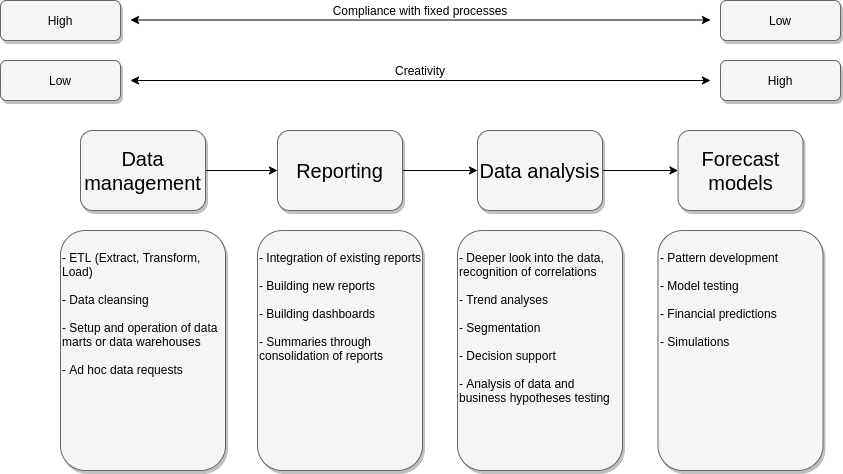
\includegraphics[width=0.8\textwidth]{levelofanalytics}
    \label{figure:levelofanalysis}
    \\
    \cite[Source: Based on][Fig. 2]{bihani2014comparative}
\end{figure}

\begin{itemize}
    \item \textbf{Management of data: }Management of various data is readily available. All relevant
    data are available and can be fed into a data warehouse. This analysis can be found in chap.
    \ref{toc:internedatenquellen} and their summaries in table \ref{tbl:klassifizierunginternedaten} and
    \ref{tbl:klassifizierungexternedaten}. The management of the data is also of immediate
    importance, as this lays the groundwork for optimizing cryptomining data centers. Since for all sub-hypotheses
    the management of the data is possible, it is also for the main hypothesis. It can be stated that the first
    stage is achievable without any problems.
    \item \textbf{Reporting: }The second stage of the use of data is the establishment of a reporting system. A reporting system
    uses existing past data to generate reports appropriate for the stakeholders in the \ac{BI} process.
    In this case, these are reports that cover the sub-hypotheses and are thus of a personnel, technical, or financial
    nature. Since this
    stage is descriptive, this is also possible according to table \ref{tbl:hypothesenanalyse} for all four subhypotheses.
    Therefore, it is possible to apply reporting for the statements of the main hypothesis. Just this stage is necessary for
    achieving the central statement of the main hypothesis ("financial optimization") centrally, because this is the basis
    for the optimization of a cryptomining data center.
    \item \textbf{Analysis of the data: }In the third step, the data is analyzed in more depth to be able to determine more correlations between the
    data and to generate more knowledge, which can be used for the optimization of data centers.
    Therefore, the main hypothesis is also found in this stage. Here the already
    existing data is used to generate statements and decision support. To this stage belong the
    analysis procedures already mentioned in chapter \ref{toc:analyseverfahrenbi}, the support for decisions and also
    the analysis of business hypotheses.
    Since this stage is again based on existing data and does not make direct predictions, this
    Stage is achievable for all sub-hypotheses. Therefore, it can be stated that the main hypothesis can also be answered positively for this stage.
    Only at this stage the actual \ac{BI} process is reached, because only at this stage the support for decisions comes into play.
    Therefore, a financial optimization of cryptomining data centers by means of
    \ac{BI} is possible in principle.
    \item \textbf{Prediction models: }The last stage is the formation of predictive models. This is the predictive part of
    \ac{BI} and lays the foundations for prescriptive \ac{BI} Systems. This stage is easily achievable for \ac{HT0.2} and \ac{HT0.4}.
    For \ac{HT0.1} and \ac{HT0.3}, the problems are entirely due to the poor predictability of bitcoin
    exchange rates. If there are improvements in this area, this level may also be achievable.
    Possible approaches to improvement are discussed in chapter \ref{toc:planungeinesbiprozessesfuereinminingrechenzentrum}
    evaluated and ultimately added to the assessment of the main hypothesis. In this course of this argumentation there is still
    no final answer to the main hypothesis to be found at this point.
\end{itemize}

In the next chapter, the statements made in this section are evaluated by means of a case study in order to obtain reliable statements about the
the hypotheses and to support and extend them by two methodologies. The focus will be on the
on the testing of the partial hypotheses in relation to the prediction models, in order to be able to answer this open part
finally.